\chapter{Resultados e Interpretación}\label{chapter:Results}

Antes de presentar los resultados, es 
importante recordar que el flujo completo de procesamiento 
(desde la sincronización y el filtrado de ruido hasta la 
detección y asignación heurística de los cantos) se diseñó con 
el fin de reconstruir con precisión las series temporales de 
vocalización de cada individuo. En este capítulo se evalúa, en 
primer lugar, la consistencia y precisión logradas por los 
algoritmos de detección y asignación micrófono-Colín, 
comparando su rendimiento 
con mediciones manuales de referencia. A continuación, se 
efectúa una comparación entre las diferentes 
estrategias heurísticas desarrolladas, con el objetivo de 
identificar fortalezas y limitaciones de cada enfoque. 
Posteriormente, se analiza la red de interacciones inferidas 
(los parámetros \(\{J_{ij}\}\)) para caracterizar la estructura 
acústica del coro. 
Finalmente, se discute la idoneidad del modelo de Ising como 
representación estadística del sistema, valorando su capacidad 
para reproducir los patrones de cantos observados.  


% region Results Eval
\section{Resultados y evaluación de los algoritmos propuestos}
\label{sec:res_asignacion}



Al aplicar el algoritmo descrito en la Sección~\ref{sec:alg_energia} sobre 
el 
\textit{dataset} preprocesado, se obtuvo, para cada hora, una 
secuencia temporal de los cantos de cada Colín. 
Un fragmento representativo de diez 
segundos de los archivos correspondientes a \texttt{20231021\_190000}
se muestra en la Figura~\ref{fig:seq}, donde puede 
apreciarse cómo el método distingue de forma coherente los 
eventos de “CO” y “LIN” en cada canal.

\begin{figure}[ht]
    \centering
    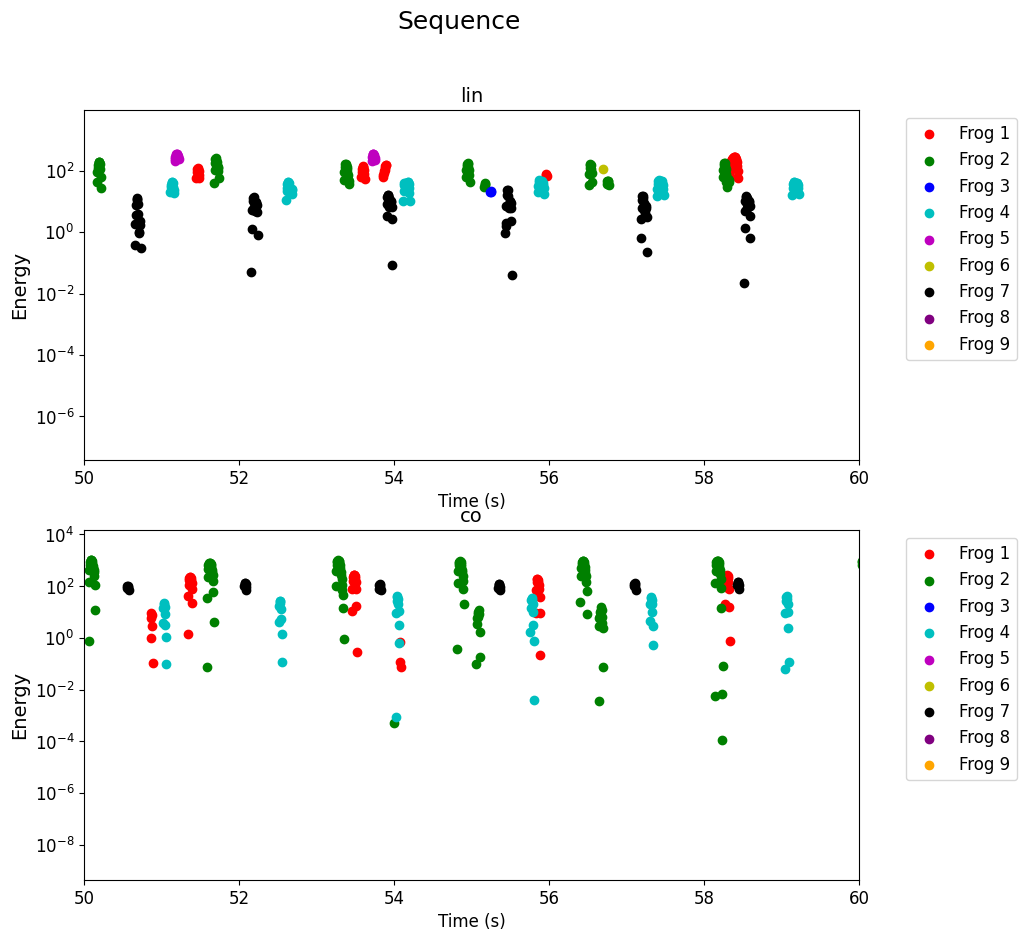
\includegraphics[width=\columnwidth]{Graphics/sequence.png}
    \caption{Fragmento de Secuencia de Cantos de los Colines en los archivos de \texttt{20231021\_190000}.}
    \label{fig:seq}
\end{figure}

En el intervalo analizado, las detecciones mantuvieron una 
periodicidad aproximada y una consistencia energética que 
parecen indicar la correcta detección y asignación de los cantos, 
condición 
imprescindible para avanzar hacia el estudio de las 
interacciones acústicas.

\subsection{Consistencia}
\label{sec:res_consistencia}

Para evaluar la consistencia del algoritmo, se realizaron diez 
ejecuciones independientes sobre el mismo conjunto de datos. En 
cada corrida se generaron nueve vectores (uno por micrófono-Colín), 
cada uno con los valores
de energía de los cantos asignados a ese micrófono, ubicados en los 
índices correspondientes a los instantes de tiempo en que fueron 
detectados los cantos. A fin de cuantificar la 
estabilidad de los resultados, se construyó una gran matriz de 
correlación cruzada entre todos los vectores provenientes de las 
diferentes ejecuciones.

La organización de la matriz siguió un orden bloque por bloque: 
primero se agruparon los vectores del micrófono “a” en cada una 
de las diez corridas, luego los del micrófono “b”, y así 
sucesivamente. De este modo, una alta correlación a lo largo de 
la diagonal principal indicaría que, para un mismo micrófono, 
las detecciones fueron reproducibles en cada ejecución.

La Figura~\ref{fig:correlation} presenta el mapa de calor de esa 
matriz. Se resaltaron en rojo las diez correlaciones más 
elevadas de cada fila. La evidente concentración de valores 
altos en la diagonal principal confirma que los vectores de 
detección correspondientes a un mismo micrófono exhibieron 
correlaciones significativamente mayores entre sí que con los 
vectores de otros canales. Este comportamiento empírico 
demuestra que el algoritmo produjo resultados coherentes y 
reproducibles.

\begin{figure}[ht]
    \centering
    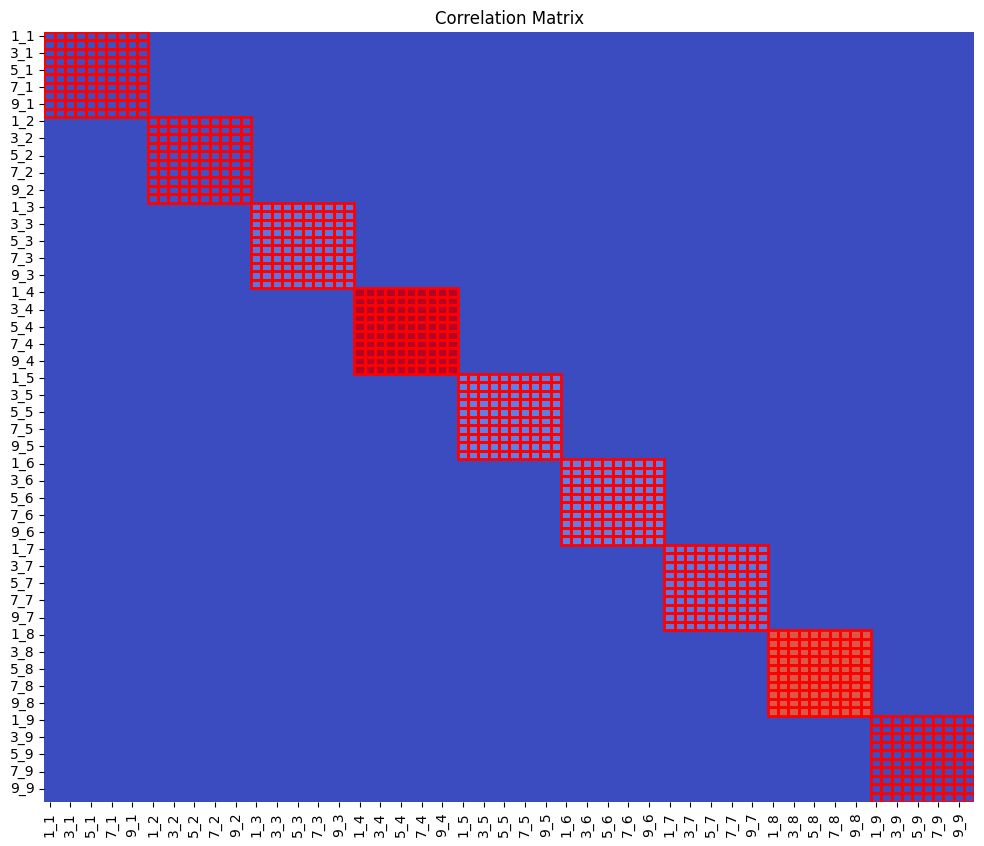
\includegraphics[width=0.7\linewidth]{Graphics/correlation_matrix.png}
    \caption{Matriz de correlación entre ejecuciones independientes del algoritmo sobre los datos de \texttt{20231021\_190000}. Los bloques diagonales de alta correlación (marcados en rojo) muestran la consistencia de las detecciones para cada micrófono.}
    \label{fig:correlation}
\end{figure}


% region Comparison
\section{Comparación entre algoritmos heurísticos}
\label{sec:res_comparacion}


Con el objetivo de validar la robustez de los métodos propuestos 
para la detección y asignación de cantos, se compararon los 
resultados obtenidos mediante ambos algoritmos heurísticos 
presentados en el Capítulo anterior. 
La Figura~\ref{fig:alg_comparison} muestra un gráfico de 
dispersión que compara los tiempos de detección de cada canto 
individual en los archivos de \texttt{20231021\_190000}, con cada 
punto representando un canto detectado por ambos algoritmos y 
coloreado según el individuo correspondiente. La línea negra 
discontinua representa la identidad \( y = x \), indicando 
perfecta coincidencia entre ambos métodos. Por simplicidad,
el algoritmo descrito en la Sección~\ref{sec:alg_energia} se
denominó \textbf{Algoritmo A} y el de la Sección~\ref{sec:alg_comportamiento},
\textbf{Algoritmo B}.

\begin{figure}[ht]
    \centering
    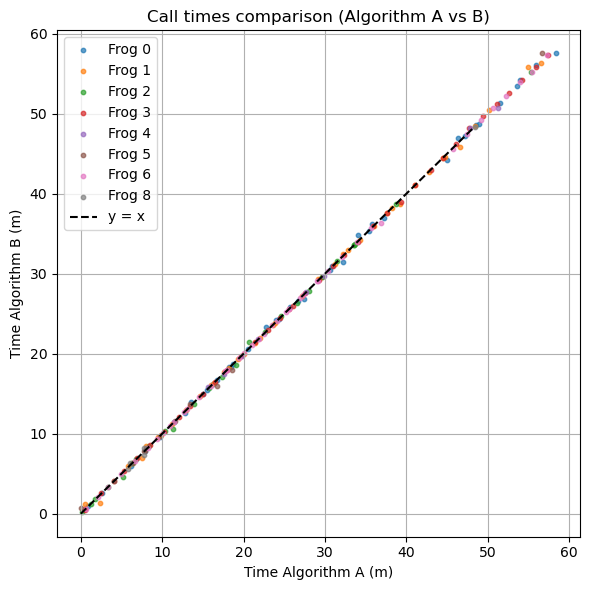
\includegraphics[width=\columnwidth]{Graphics/times_comparison.png}
    \caption{Comparación entre los tiempos de detección de cantos por los algoritmos A (energías relativas) y B (comportamiento de la especie) sobre los datos de \texttt{20231021\_190000}.}
    \label{fig:alg_comparison}
\end{figure}

Como puede observarse, la mayoría de los puntos se alinean con 
alta precisión sobre la recta de identidad, lo que indica un 
alto grado de concordancia entre ambos algoritmos en cuanto a 
los instantes de detección. Este resultado sugiere que, a pesar 
de basarse en supuestos distintos, ambos métodos producen 
secuencias temporales coherentes, lo cual refuerza la validez 
de los procedimientos desarrollados.

Para cuantificar con mayor precisión esta similitud, se realizó 
un ajuste lineal entre los tiempos de detección generados por 
ambos algoritmos para cada canal (o micrófono) por separado. Se 
calculó el coeficiente de determinación \( R^2 \), métrica 
comúnmente empleada para evaluar la calidad del ajuste de 
modelos lineales \cite{nagelkerke1991note}. Un valor cercano a 
\( R^2 = 1 \) reflejan una alta correlación.

La Tabla~\ref{tab:r2_results} resume los valores obtenidos de 
\( R^2 \) para los nueve canales analizados. En ocho de los 
casos se obtuvo un valor de \( R^2 = 1.00 \), indicando un 
solapamiento perfecto entre los resultados. Solo uno de los 
canales presentó un valor ligeramente inferior (\( R^2 = 0.99 \)), 
lo cual sigue siendo una indicación de coincidencia 
prácticamente total.

\begin{table}[ht]
    \centering
    \caption{Coeficientes de determinación \( R^2 \) del ajuste lineal entre algoritmos A y B por micrófono.}
    \label{tab:r2_results}
    \begin{tabular}{lc}
        \toprule
        \textbf{Micrófono} & \textbf{\( R^2 \)} \\
        \midrule
        \texttt{20231021\_190000a} & 1.00 \\
        \texttt{20231021\_190000b} & 1.00 \\
        \texttt{20231021\_190000c} & 1.00 \\
        \texttt{20231021\_190000d} & 1.00 \\
        \texttt{20231021\_190000e} & 0.999 \\
        \texttt{20231021\_190000f} & 1.00 \\
        \texttt{20231021\_190000g} & 1.00 \\
        \texttt{20231021\_190000h} & 1.00 \\
        \texttt{20231021\_190000i} & 1.00 \\
        \bottomrule
    \end{tabular}
\end{table}

Estos resultados corroboran que los algoritmos propuestos no 
solo son internamente consistentes, sino que ofrecen una 
detección altamente reproducible y concordante, 
independientemente del criterio heurístico considerado. 
Esta coincidencia refuerza la fiabilidad de las secuencias de 
canto extraídas, base fundamental para el análisis posterior de 
las interacciones acústicas en el sistema.

% region Ising
\section{Análisis de las interacciones inferidas \(\{J_{ij}\}\)}
\label{sec:res_interacciones}


La red de interacciones acústicas entre individuos fue inferida 
mediante el modelo de Ising descrito en el Capítulo anterior, 
utilizando configuraciones binarizadas de cantos. 
Este modelo permitió 
cuantificar la fuerza de acoplamiento entre pares de individuos, 
interpretada como una medida de influencia mutua en la emisión 
de vocalizaciones. 

En la Figura~\ref{fig:jij} se muestra la matriz simétrica 
\( J_{ij} \) obtenida para los datos de \texttt{20232110\_190000}. 
En ella, cada entrada 
representa la magnitud y dirección de la interacción inferida 
entre los individuos \( i \) y \( j \). Se observa una 
estructura dispersa, con varios acoplamientos claramente 
distintos de cero, lo que sugiere la existencia de vínculos 
acústicos no triviales entre ciertos miembros del coro. Las 
intensidades positivas indican una tendencia a la co-emisión 
simultánea, mientras que los valores negativos reflejan 
inhibición recíproca.

\begin{figure}[htbp]
    \centering
    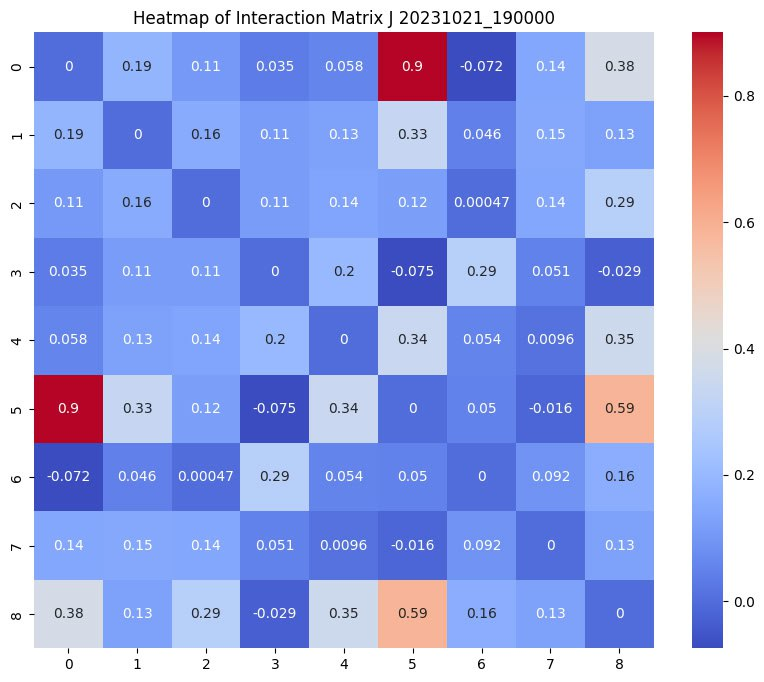
\includegraphics[width=0.7\linewidth]{Graphics/matrix_jij.jpg}
    \caption{Matriz de interacciones \( J_{ij} \) inferida para el \texttt{20231021\_190000}.}
    \label{fig:jij}
\end{figure}

Con el fin de facilitar la interpretación estructural de estas 
relaciones, se construyó un grafo no dirigido donde cada nodo 
representa a un individuo (o micrófono) y las aristas indican 
la existencia de interacciones significativas. En particular, 
se utilizó una línea continua para aquellas interacciones cuya 
magnitud supera el umbral de 0.5, y una línea discontinua para 
aquellas en el rango entre 0.3 y 0.5. Las conexiones cuya 
magnitud resultó inferior a este último valor se consideraron 
insignificantes y fueron omitidas del grafo para mejorar la 
claridad visual. El resultado se presenta en la 
Figura~\ref{fig:graph}.

\begin{figure}[ht]
    \centering
    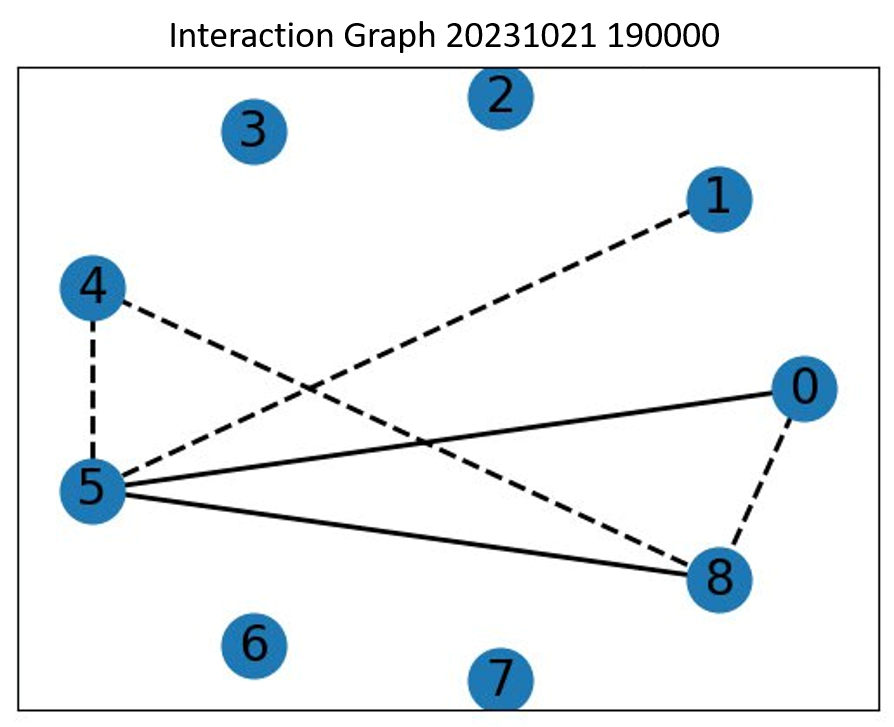
\includegraphics[width=0.7\linewidth]{Graphics/corr_graph.png}
    \caption{Grafo de interacciones correspondiente al \texttt{20231021\_190000}.}
    \label{fig:graph}
\end{figure}

Como análisis exploratorio adicional, se aplicó el mismo 
procedimiento de inferencia sobre tres intervalos horarios 
consecutivos de la misma noche (\texttt{20231021\_180000}, \texttt{20231021\_190000}, \texttt{20231021\_200000}). 
La Figura~\ref{fig:jij_evol} 
muestra la evolución de las matrices \( J_{ij} \) a lo largo 
de estas tres horas. Se observa que varias de las interacciones 
más fuertes (especialmente aquellas con valores superiores a 
0.5) se mantienen estables en el tiempo. Un ejemplo destacado es 
la interacción entre los individuos indexados como 0 y 5, que 
presenta una magnitud elevada y sostenida a lo largo del 
intervalo temporal analizado.

\begin{figure}[ht]
    \centering
    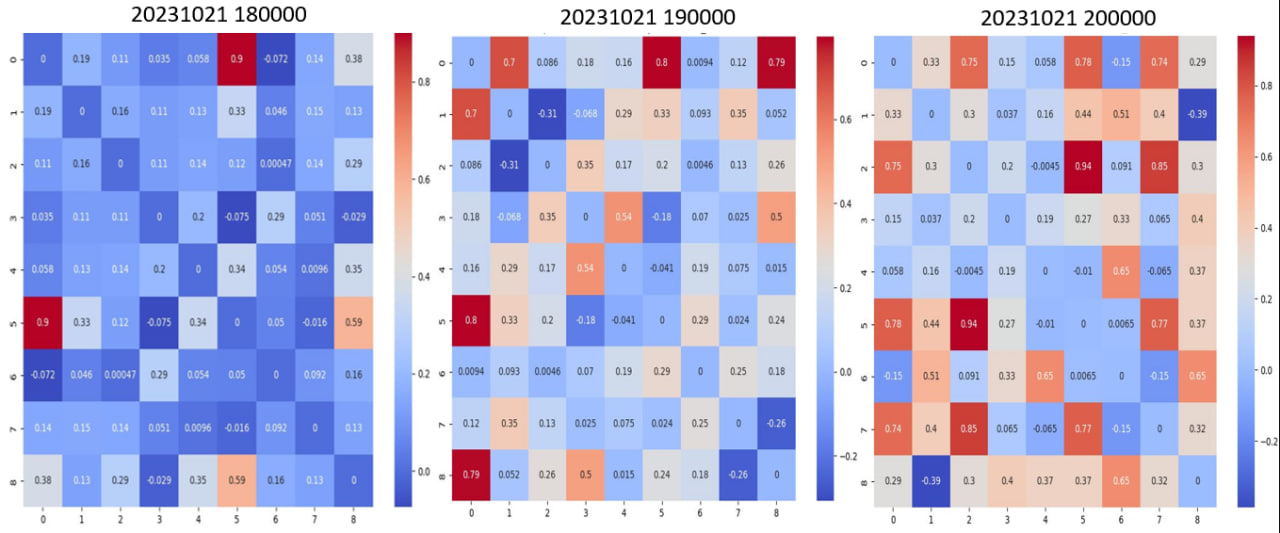
\includegraphics[width=\columnwidth]{Graphics/3_matrixs.jpg}
    \caption{Evolución de la matriz \( J_{ij} \) durante tres horas consecutivas (\texttt{20231021\_180000}, \texttt{20231021\_190000}, \texttt{20231021\_200000}).}
    \label{fig:jij_evol}
\end{figure}

Este patrón de persistencia fue también evidente en la 
representación gráfica de las redes inferidas, ilustradas en la 
Figura~\ref{fig:graph_evol}. La presencia continua de ciertas 
aristas a lo largo del tiempo sugiere la existencia de 
relaciones acústicas recurrentes y posiblemente funcionales 
entre algunos individuos. Dichos vínculos podrían reflejar 
mecanismos de coordinación o competencia territorial que 
merecen ser explorados en mayor profundidad en estudios futuros.

\begin{figure}[ht]
    \centering
    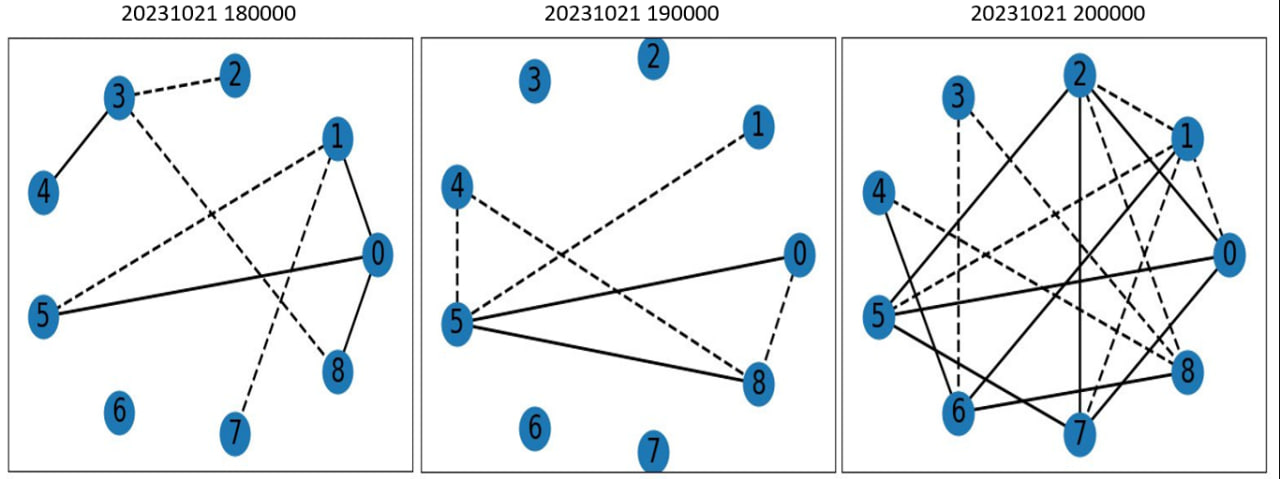
\includegraphics[width=\columnwidth]{Graphics/3_graphs.jpg}
    \caption{Evolución temporal de los grafos de interacciones inferidas para tres horas consecutivas (\texttt{20231021\_180000}, \texttt{20231021\_190000}, \texttt{20231021\_200000}).}
    \label{fig:graph_evol}
\end{figure}

Bajo el supuesto de que el modelo de Ising logra cantificar correctamente
las interacciones del sistema, estos hallazgos refuerzan la hipótesis de 
que los coros de 
\emph{E.\,eileenae} exhiben una estructura interna no aleatoria.


% region Idoneidad
\section{Análisis de idoneidad del modelo de Ising}
\label{sec:res_idoneidad}


Para evaluar la capacidad predictiva del modelo de Ising, se 
compararon sus estimaciones de la tasa de aparición de patrones 
de canto con las obtenidas bajo un modelo independiente en el 
que se asumen que cada Colín actúa sin influencia de los otros individuos 
\cite{schneidman2006weak}.

En la Figura~\ref{fig:ising_vs_indep} se presentan, en escala logarítmica, 
los patrones observados frente a los patrones predichos por 
ambos modelos para dos ventanas horarias distintas: \texttt{20231021\_190000}
y \texttt{20231021\_040000}. Cada punto corresponde a la frecuencia de un patrón 
particular de activación de espines (combinación de individuos 
cantando simultáneamente). La línea punteada \(y=x\) indica 
coincidencia perfecta entre observación y predicción.

\begin{figure}[ht]
    \centering
    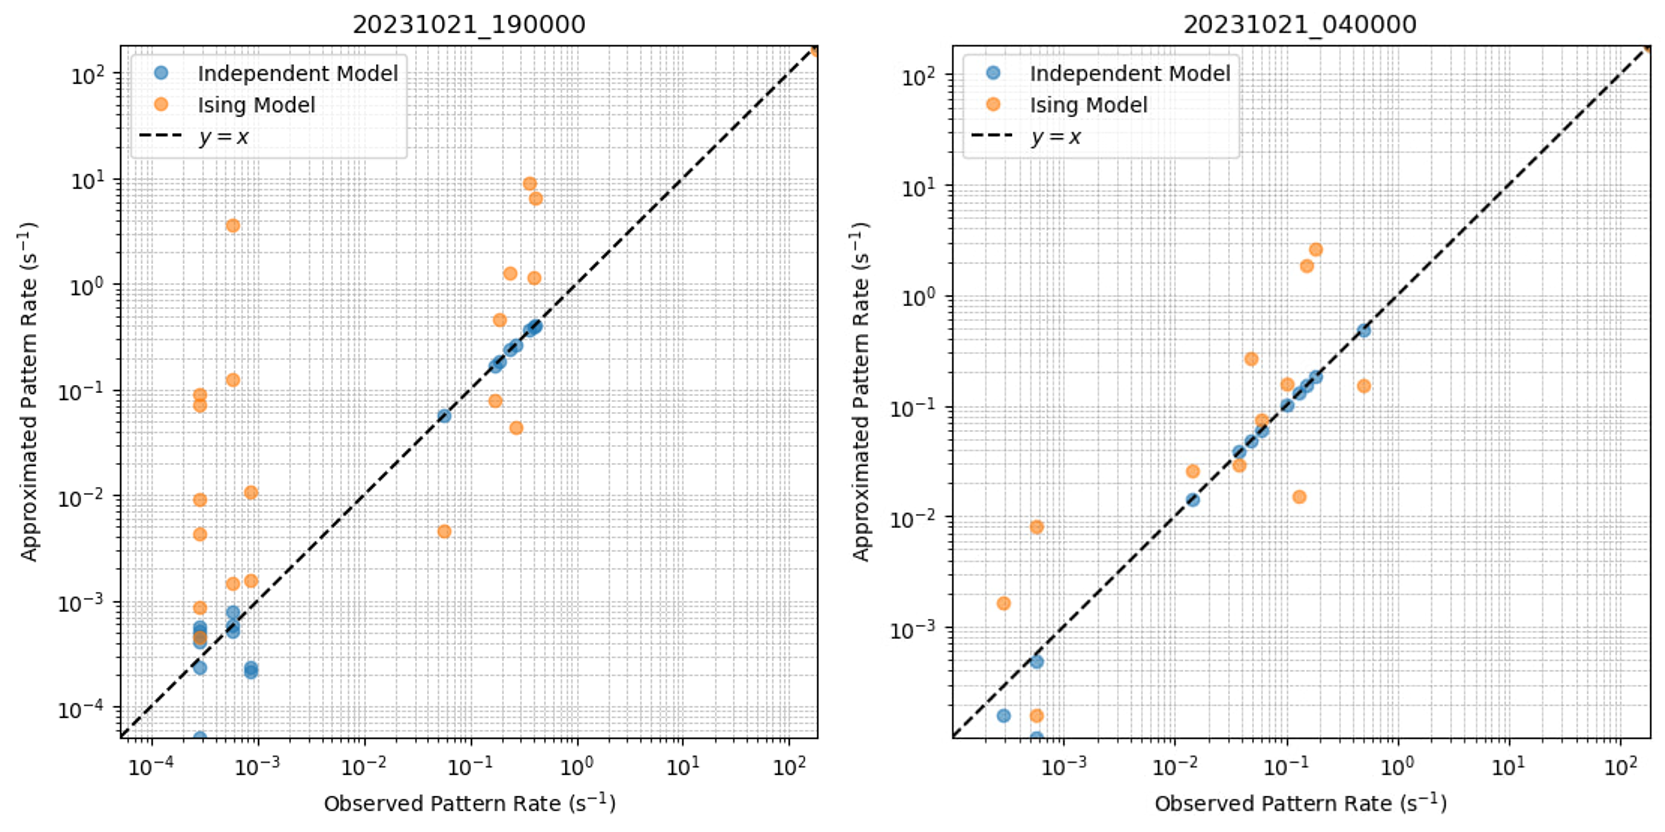
\includegraphics[width=\columnwidth]{Graphics/isingvsindependent.png}
    \caption{Tasa de aparición de patrones de canto observada versus predicha por el modelo independiente (azul) y el modelo de Ising (naranja) para las grabaciones de \texttt{20231021\_190000} (izq.) y \texttt{20231021\_040000} (der.).}
    \label{fig:ising_vs_indep}
\end{figure}

Contrariamente a lo esperado, el modelo independiente mostró una 
correspondencia más estrecha con las tasas observadas que el 
modelo de Ising, cuya predicción se desvió considerablemente en 
varios patrones de baja frecuencia. Este resultado sugiere al 
menos tres posibles interpretaciones: (1) las interacciones 
acústicas entre individuos podrían ser efectivamente débiles o 
nulas durante las ventanas analizadas, (2) el modelo de Ising, 
en su forma estacionaria y de segundo orden, podría no capturar 
adecuadamente la dinámica temporal o no lineal de los coros, o 
(3) la escasez de datos para patrones raros impide una estimación 
fiable de los parámetros de interacción.

En conjunto, estos hallazgos indican que, para el conjunto de 
grabaciones y la metodología empleada, el supuesto de 
independencia entre Colines resulta tan (o más) efectivo que el 
modelo de Ising para describir la distribución de patrones de 
canto. No obstante, la presencia de acoplamientos significativos 
observados en Sección~\ref{sec:res_interacciones} sugiere que 
podría ser necesaria una extensión del modelo (por ejemplo, 
incorporando términos de orden superior, efectos no 
estacionarios o dependencias temporales explícitas) para 
capturar plenamente la complejidad del comportamiento grupal de 
\emph{E.\,eileenae}.
